\documentclass[12pt,a4paper]{article}
% This text is inserted in the beginning of all
% LaTex and Tex files I create.
%
% File created: Tue Sep 26 2017
% File name:    report_template.tex
% Path:         /home/name/Classes/AMPIII/Template/
%
% Name
% Sept, 2017
%

%recommended by fancyhdr package
\setlength{\headheight}{14.49998pt}
\addtolength{\topmargin}{-2.49998pt}

% include a minimal set of useful packages

\usepackage{float}
\usepackage{graphicx}
\usepackage{subfiles}
\usepackage{amsfonts} 
\usepackage{amssymb}
\usepackage{amsmath}
\usepackage{lastpage}
\usepackage{fancyhdr}
\usepackage{caption}
\usepackage{subcaption}
\usepackage[table,xcdraw,dvipsnames]{xcolor}
\usepackage{cancel}
\usepackage{xcolor, soul}
\sethlcolor{Lavender}
\newcommand{\mathcolorbox}[2]{\colorbox{#1}{$\displaystyle #2$}}
\usepackage{amsmath,amssymb}
\usepackage{pdfpages}
\usepackage[dvipsnames]{xcolor}
\usepackage{tcolorbox}
\usepackage[a4paper,margin=2cm]{geometry}
\tcbuselibrary{minted,breakable,xparse,skins}

\DeclareTCBListing{mintedbox}{O{}m!O{}}{%
  breakable=true,
  listing engine=minted,
  listing only,
  minted language=#2,
  minted style=default,
  minted options={%
    linenos,
    gobble=0,
    breaklines=true,
    breakafter=,,
    fontsize=\small,
    numbersep=8pt,
    #1},
  boxsep=0pt,
  left skip=0pt,
  right skip=0pt,
  left=35pt,
  right=0pt,
  top=3pt,
  bottom=3pt,
  arc=5pt,
  leftrule=0pt,
  rightrule=0pt,
  bottomrule=2pt,
  toprule=2pt,
  colback=Lavender!15,
  colframe=Lavender,
  enhanced,
  overlay={%
    \begin{tcbclipinterior}
    \fill[Lavender!50!white] (frame.south west) rectangle ([xshift=30pt]frame.north west);
    \end{tcbclipinterior}},
  #3}

\AtBeginEnvironment{quote}{\itshape}
% PUT YOUR TITLE AND NAME HERE
\newcommand{\titlestr}{TITLE}
\newcommand{\shorttitlestr}{PHYSICAL CHEMISTRY III EXP 3 LAB REPORT}
\newcommand{\authorstr}{Mei He} % INSERT YOUR NAME(S)
\usepackage[backend=biber,style=chem-acs]{biblatex}
\addbibresource{bib_file.bib}
\begin{document}

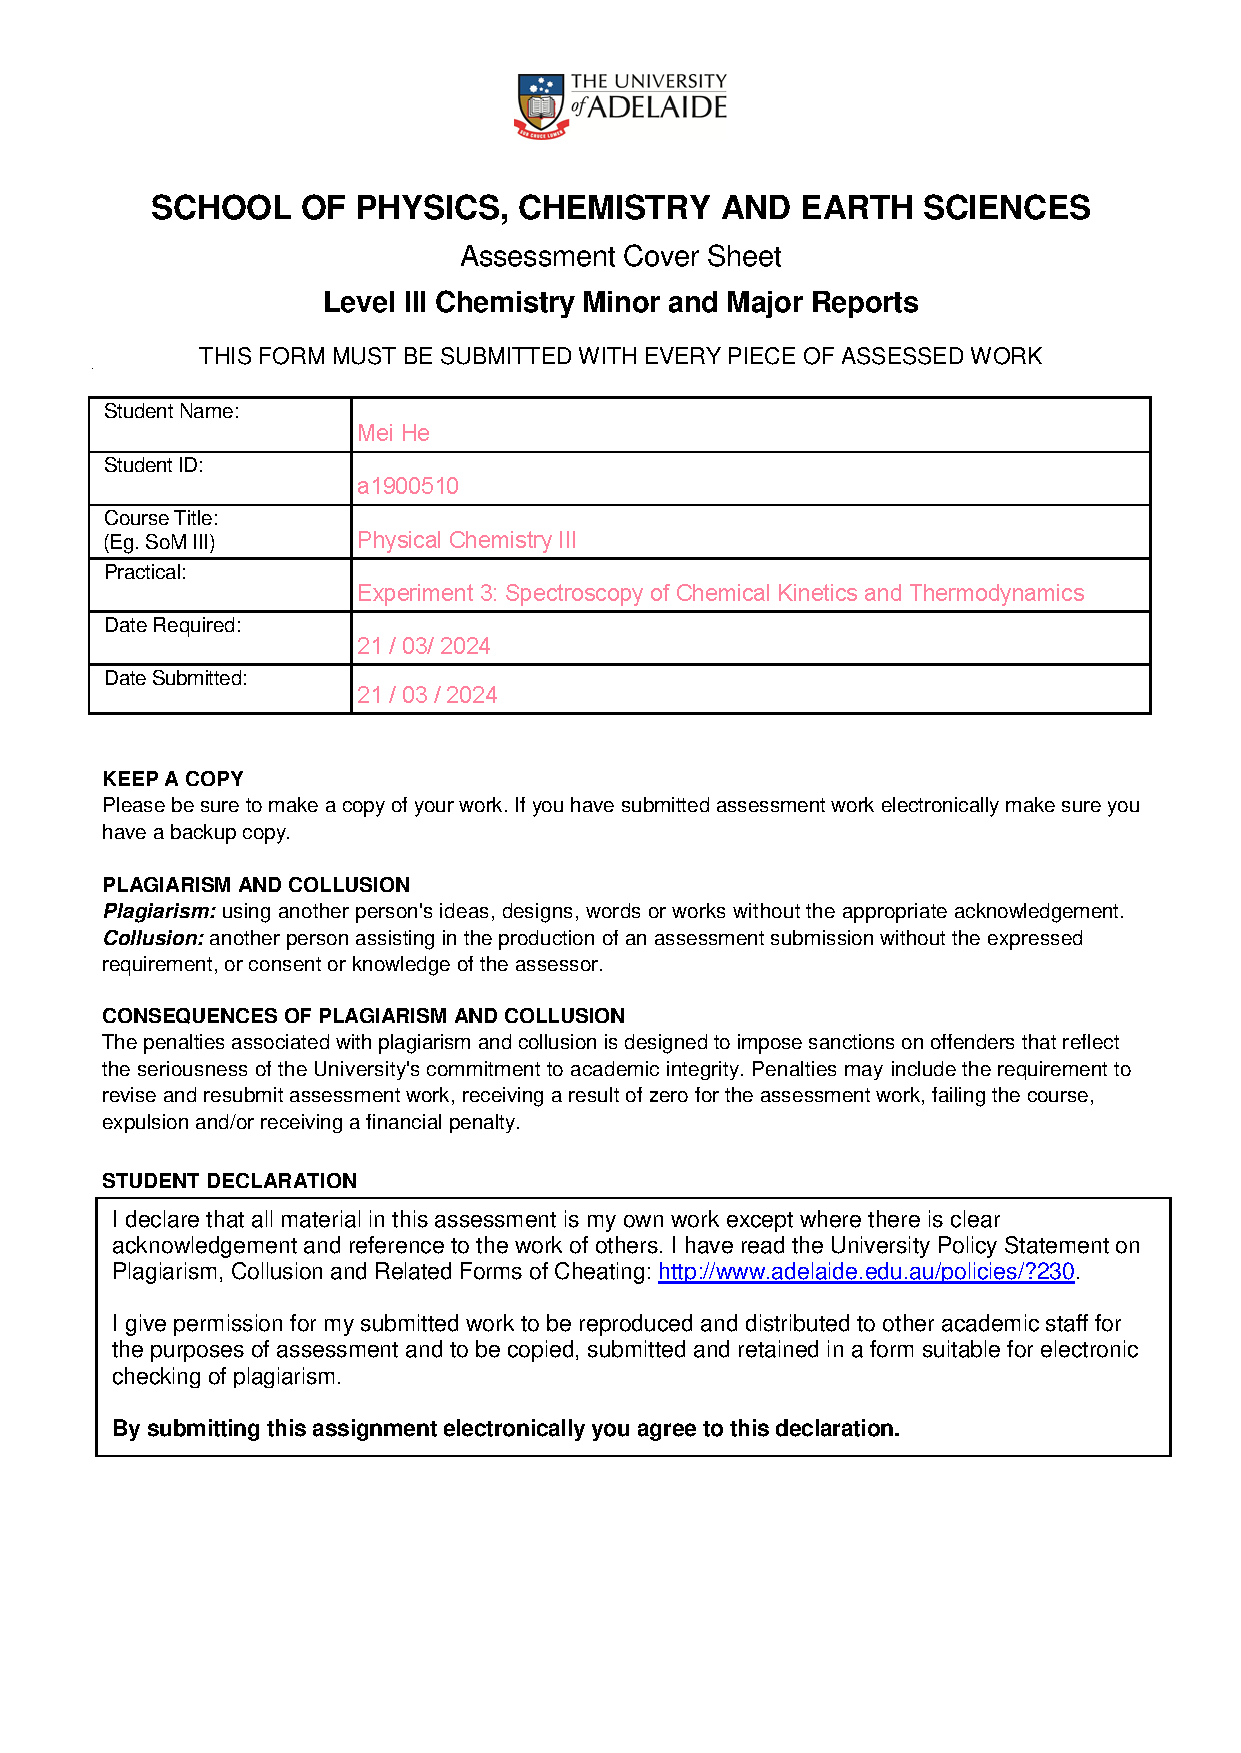
\includepdf[pages=-]{exp3_cover.pdf}


%%%%%%%%%%%%%%%%%%%%%%%%%%%%%%555
% title page
\begin{titlepage}
  \centering
  
  {\LARGE \titlestr \par}

  \vspace{1cm}
  {\Large \authorstr \par}

  {\bf A1900510}

  \vspace{1cm}
Thursday March 7 2024     % PUT YOUR DATE HERE

  \vspace{1cm}
  Report submitted for
  {\bf Physical Chemistry III}
  at the University of Adelaide. \textbf{Due 23:59pm March 21st 2024}

  \vspace{1cm}
    \begin{abstract}
        chuck abstract here
    \end{abstract}
  \vspace{1cm}
  \tableofcontents
  \listoffigures

  \vfill
\end{titlepage}

% put headings on each page
\pagestyle{fancy}
\fancyhf{}
\rhead{\shorttitlestr}
\lhead{\authorstr}
\rfoot{Page \thepage\ of \pageref{LastPage}}
\renewcommand{\headrulewidth}{1pt}

%%%%%%%%%%%%%%%%%%%%%%%%%%%%%%555
% main report
\clearpage


%%%%%%%%%%%%%%%%%%%%%%%%%%%%%%555
% intro
\section{Introduction}
\subfile{intro.tex}
A short introductory section incorporating the experimental aims. You may include figures and diagrams, but
these should be prepared yourself or properly attributed.
%%%%%%%%%%%%%%%%%%%%%%%%%%%%%%555
% experiment
\section{Experiment}
An experimental section. The experimental section will have a more experiment specific component but adequate 
details of what was done in the practical still need to be provided
\subfile{experiment}



%%%%%%%%%%%%%%%%%%%%%%%%%%%%%%555
% Results
\section{Results \& Discussion}
\subfile{results_discussion}

% concl
\section{Conclusion}
\subfile{conclusion}


%%%%%%%%%%%%%%%%%%%%%%%%%%%%%%555
% references
\addcontentsline{toc}{section}{References}

\printbibliography

\newpage
\section{Appendix}
\subfile{appx}
\end{document}


 